\subsection{Rockey dongle: finding unknown algorithm using only input/output pairs and Z3 SMT solver}

(This article was first published in August 2012 in my blog: \url{http://blog.yurichev.com/node/71}).

Some smartcards can execute Java or .NET code - that's the way to hide your sensitive algorithm into chip that very hard to break (decapsulate).
For example, one may encrypt/decrypt data files by hidden crypto algorithm rendering software piracy of such software nearly impossible.

That's what called Black box in mathematics\footnote{\url{http://en.wikipedia.org/wiki/Black\_box}}.

Some software protection dongles offers this functionality too.

One example is Rockey 4 (\href{http://www.rockey.nl/en/rockey.html}{www.rockey.nl}).

\begin{figure}[H]
\centering
%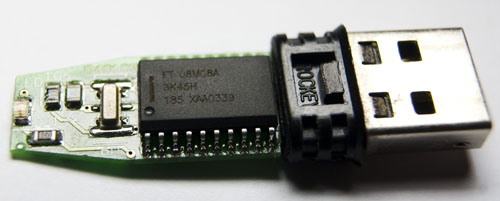
\includegraphics[scale=0.66]{rockey_4.jpg}
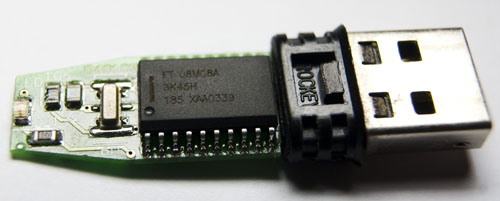
\includegraphics[scale=2]{rockey_4.jpg}
\caption{Rockey 4 dongle}
\end{figure}

This is small dongle connected via USB. Is contain some user-defined memory but also memory for user algorithms.

The virtual (toy) CPU for these algorithms is very simple: it offer only 8 16-bit registers (however, only 4 can be set and read) and 8 operations (add, subtract, cyclic left shift, multiplication, or, xor, and, negate).

Second instruction argument can be a constant (from 0 to 63) instead of register.

Each algorithm is described by string like \colorbox{light-gray}{\TT{A=A+B, B=C*13, D=D\^{}A, C=B*55, C=C\&A, D=D|A, A=A*9, A=A\&B}}.

There are no stack, conditional/unconditional jumps, etc.

Each algorithm, obviously, can't have side effects, so they are actually pure functions
\footnote{\url{http://en.wikipedia.org/wiki/Pure_function}} and their results can be 
memoized\footnote{\url{http://en.wikipedia.org/wiki/Memoization}}.

By the way, as it was mentioned in Rockey 4 manual, first and last instruction cannot have constants. Maybe that's because these fields used for some internal data: each algorithm start and end should be marked somehow internally anyway.

Would it be possible to reveal hidden impossible-to-read algorithm only by recording input/output dongle traffic?

Common sense tell us "no". But we can try anyway.

Since, my goal wasn't to break into some Rockey-protected software, I was interesting only in limits (which algorithms could we find), so I make some things simpler: we will work with only 4 16-bit registers, and there will be only 6 operations (add, subtract, multiplication, or, xor, and).

Let's first calculate, how much information will be used in brute-force case.

There are 384 of all possible instructions in format reg=reg,op,reg for 4 registers and 6 operations, and also 6144 instructions in format reg=reg,op,constant. Remember that constant limited to 63 as maximal value? That help us for a little.

So, here 6528 all possible instructions. This mean, there are about 11854977354713530368 5-instruction algorithms. Wow! That's too much. I don't even know a precise name for such numbers. That's about 11 quintillions (thanks to Wikipedia).

Now let's try to use real heavy machinery:

\begin{framed}
\begin{quotation}
Constraint satisfaction problems (CSPs) are mathematical problems defined as a set of objects whose state must satisfy a number of constraints or limitations. CSPs represent the entities in a problem as a homogeneous collection of finite constraints over variables, which is solved by constraint satisfaction methods. CSPs are the subject of intense research in both artificial intelligence and operations research, since the regularity in their formulation provides a common basis to analyze and solve problems of many unrelated families. CSPs often exhibit high complexity, requiring a combination of heuristics and combinatorial search methods to be solved in a reasonable time. The boolean satisfiability problem (SAT), the Satisfiability Modulo Theories (SMT) and answer set programming (ASP) can be roughly thought of as certain forms of the constraint satisfaction problem.
\end{quotation}
\end{framed}\footnote{\url{http://en.wikipedia.org/wiki/Constraint_satisfaction_problem}}

... and:

\begin{framed}
\begin{quotation}
In computer science and mathematical logic, the Satisfiability Modulo Theories (SMT) problem is a decision problem for logical formulas with respect to combinations of background theories expressed in classical first-order logic with equality. Examples of theories typically used in computer science are the theory of real numbers, the theory of integers, and the theories of various data structures such as lists, arrays, bit vectors and so on. SMT can be thought of as a form of the constraint satisfaction problem and thus a certain formalized approach to constraint programming.
\end{quotation}
\end{framed}\footnote{\url{http://en.wikipedia.org/wiki/Satisfiability_Modulo_Theories}}

I'll use Z3 Theorem Prover
\footnote{\url{http://research.microsoft.com/en-us/um/redmond/projects/z3/}} from Microsoft Research with excellent 
Python bindings, working like SMT solver.

It can be said, SMT solver is just solver of very big system of equations. 
By the way, its sibling SAT solver is intended for solving very big boolean system of equations.

Needless to say, a lot of tasks can be expressed as system of equations. 
One very simple example is Sudoku: \url{https://sites.google.com/site/modante/sudokusolver}

So let's back to our toy CPU inside of Rockey 4 dongle.

How can we express each instruction as system of equations? While remembering some school math, I wrote this:

% WAT THIS IS?
Function one\_step()=

\begin{lstlisting}
Each Bx is integer, but may be only 0 or 1.

# only one of B1..B4 and B5..B9 can be set
reg1=B1*A + B2*B + B3*C + B4*D
reg_or_constant2=B5*A + B6*B + B7*C + B8*D + B9*constant
reg1 should not be equal to reg_or_constant2

# Only one of B10..B15, can be set
result=result+B10*(reg1*reg2)
result=result+B11*(reg1^reg2)
result=result+B12*(reg1+reg2)
result=result+B13*(reg1-reg2)
result=result+B14*(reg1|reg2)
result=result+B15*(reg1&reg2)

B16 - true if register isn't updated in this part
B17 - true if register is updated in this part
(B16 cannot be equal to B17)
A=B16*A + B17*result
B=B18*A + B19*result
C=B20*A + B21*result
D=B22*A + B23*result
\end{lstlisting}

That's how we can express each instruction in algorithm.

5-instructions algorithm can be expressed like this: one\_step (one\_step (one\_step (one\_step (one\_step (input\_registers)))))

Let's also add five known input/output pairs and we'll get system of equations like this:

\begin{lstlisting}
one_step (one_step (one_step (one_step (one_step (input_1)))))==output_1
one_step (one_step (one_step (one_step (one_step (input_2)))))==output_2
one_step (one_step (one_step (one_step (one_step (input_3)))))==output_3
one_step (one_step (one_step (one_step (one_step (input_4)))))==output_4
.. etc
\end{lstlisting}

So the question now is to find about 5*23 boolean values satisfying known input/output pairs.

I wrote small utility to probe Rockey 4 algorithm with random numbers, it produce results in form:

\begin{lstlisting}
RY_CALCULATE1: (input) p1=30760 p2=18484 p3=41200 p4=61741 (output) p1=49244 p2=11312 p3=27587 p4=12657
RY_CALCULATE1: (input) p1=51139 p2=7852 p3=53038 p4=49378 (output) p1=58991 p2=34134 p3=40662 p4=9869
RY_CALCULATE1: (input) p1=60086 p2=52001 p3=13352 p4=45313 (output) p1=46551 p2=42504 p3=61472 p4=1238
RY_CALCULATE1: (input) p1=48318 p2=6531 p3=51997 p4=30907 (output) p1=54849 p2=20601 p3=31271 p4=44794
\end{lstlisting}

p1/p2/p3/p4 are just another names for A/B/C/D registers.

Now let's start with Z3. We will need to express Rockey 4 toy CPU in Z3Py (Z3 for Python) terms.

It can be said, my Python script is divided into two parts: 

\begin{itemize}
\item
constraint definitions (like, "output\_1 should be n for input\_1=m", "constant cannot be greater than 64", etc); 

\item
functions constructing system of equations.
\end{itemize}

This piece of code define some kind of "structure" consisting of 4 named 16-bit variables, each represent register in our toy CPU.

\begin{lstlisting}
Registers_State=Datatype ('Registers_State')
Registers_State.declare('cons', ('A', BitVecSort(16)), ('B', BitVecSort(16)), ('C', BitVecSort(16)), ('D', BitVecSort(16)))
Registers_State=Registers_State.create()
\end{lstlisting}

These enumarations define two new types (or "sorts" in Z3's terminology):

\begin{lstlisting}
Operation, (OP_MULT, OP_MINUS, OP_PLUS, OP_XOR, OP_OR, OP_AND) = EnumSort('Operation', ('OP_MULT', 'OP_MINUS', 'OP_PLUS', 'OP_XOR', 'OP_OR', 'OP_AND'))

Register, (A, B, C, D) = EnumSort('Register', ('A', 'B', 'C', 'D'))
\end{lstlisting}

This part is very important, it define all variables in our system of equations. 
op\_step is type of operation in instruction. reg\_or\_constant is selector between register or constant in second 
argument --- False if register and True if constant. 
reg\_step is register assigned in this instruction. 
reg1\_step and reg2\_step are just registers at arg1 and arg2. 
constant\_step is constant (in case it's used in instruction instead of arg2).

\begin{lstlisting}
op_step=[Const('op_step%s' % i, Operation) for i in range(STEPS)]
reg_or_constant_step=[Bool('reg_or_constant_step%s' % i) for i in range(STEPS)]
reg_step=[Const('reg_step%s' % i, Register) for i in range(STEPS)]
reg1_step=[Const('reg1_step%s' % i, Register) for i in range(STEPS)]
reg2_step=[Const('reg2_step%s' % i, Register) for i in range(STEPS)]
constant_step = [BitVec('constant_step%s' % i, 16) for i in range(STEPS)]
\end{lstlisting}

Adding constraints is very simple. Remember, I wrote that each constant cannot be larger than 63?

\begin{lstlisting}
# according to Rockey 4 dongle manual, arg2 in first and last instructions cannot be a constant
s.add (reg_or_constant_step[0]==False)
s.add (reg_or_constant_step[STEPS-1]==False)

...

for x in range(STEPS):
   s.add (constant_step[x]>=0, constant_step[x]<=63)
\end{lstlisting}

Input/output values are added as constraints too.

Now let's see how to construct our system of equations:

\begin{lstlisting}
# Register, Registers_State -> int
def register_selector (register, input_registers):
    return If(register==A, Registers_State.A(input_registers),
           If(register==B, Registers_State.B(input_registers), 
           If(register==C, Registers_State.C(input_registers), 
           If(register==D, Registers_State.D(input_registers), 
                           0)))) # default
\end{lstlisting}

This function returning corresponding register value from "structure". 
Needless to say, the code above is not executed. 
If() is Z3Py function. 
The code only declares the function, which will be used in another. 
By the way, expression declaration resembling LISP language in some way.

Here is another function where register\_selector() used:

\begin{lstlisting}
# Bool, Register, Registers_State, int -> int
def register_or_constant_selector (register_or_constant, register, input_registers, constant): 
    return If(register_or_constant==False, register_selector(register, input_registers), constant)
\end{lstlisting}

The code here is never executed too. 
It only construct one small piece of very big expression. 
But for the sake of simplicity, one can think all these functions will be called during bruteforce search.

\begin{lstlisting}
# Operation, Bool, Register, Register, Int, Registers_State -> int
def one_op (op, register_or_constant, reg1, reg2, constant, input_registers):
    arg1=register_selector(reg1, input_registers)
    arg2=register_or_constant_selector (register_or_constant, reg2, input_registers, constant)
    return If(op==OP_MULT,   arg1*arg2,
           If(op==OP_MINUS,  arg1-arg2,
           If(op==OP_PLUS,   arg1+arg2, 
           If(op==OP_XOR,    arg1^arg2, 
           If(op==OP_OR,     arg1|arg2, 
           If(op==OP_AND,    arg1&arg2, 
                          0)))))) # default
\end{lstlisting}

Here is expression describing each instruction. 
Register assigned is instruction is substitued with new\_val, 
while all other registers are copied from input register's state:

\begin{lstlisting}
# Bool, Register, Operation, Register, Register, Int, Registers_State -> Registers_State
def one_step (register_or_constant, register_assigned_in_this_step, op, reg1, reg2, constant, input_registers):
    new_val=one_op(op, register_or_constant, reg1, reg2, constant, input_registers)
    return If (register_assigned_in_this_step==A, Registers_State.cons (new_val,
                                                                        Registers_State.B(input_registers), 
                                                                        Registers_State.C(input_registers), 
                                                                        Registers_State.D(input_registers)),
           If (register_assigned_in_this_step==B, Registers_State.cons (Registers_State.A(input_registers), 
                                                                        new_val,
                                                                        Registers_State.C(input_registers),
                                                                        Registers_State.D(input_registers)), 
           If (register_assigned_in_this_step==C, Registers_State.cons (Registers_State.A(input_registers), 
                                                                        Registers_State.B(input_registers), 
                                                                        new_val,
                                                                        Registers_State.D(input_registers)), 
           If (register_assigned_in_this_step==D, Registers_State.cons (Registers_State.A(input_registers), 
                                                                        Registers_State.B(input_registers), 
                                                                        Registers_State.C(input_registers), 
                                                                        new_val),
                                                  Registers_State.cons(0,0,0,0))))) # default
\end{lstlisting}

This is the last function describing whole n-step program:

\begin{lstlisting}
def program(input_registers, STEPS):
    cur_input=input_registers
    for x in range(STEPS):
        cur_input=one_step (reg_or_constant_step[x], reg_step[x], op_step[x], reg1_step[x], reg2_step[x], constant_step[x], cur_input)
    return cur_input
\end{lstlisting}

Again, for the sake of simplicity, it can be said, now Z3 will try each possible registers/operations/constants against this expression to find such combination which satisfy input/output pairs. 
But it's not true. 
As far as I right, Z3 use DPLL algorithm\footnote{\url{http://en.wikipedia.org/wiki/DPLL_algorithm}}.

Now let's start with very simple 3-step algorithm: "B=A\^{}D, C=D*D, D=A*C". Please note: register A left unchanged.
I programmed Rockey 4 dongle with it and recorded algorithm outputs:

\begin{lstlisting}
RY_CALCULATE1: (input) p1=8803 p2=59946 p3=36002 p4=44743 (output) p1=8803 p2=36004 p3=7857 p4=24691
RY_CALCULATE1: (input) p1=5814 p2=55512 p3=52155 p4=55813 (output) p1=5814 p2=52403 p3=33817 p4=4038
RY_CALCULATE1: (input) p1=25206 p2=2097 p3=55906 p4=22705 (output) p1=25206 p2=15047 p3=10849 p4=43702
RY_CALCULATE1: (input) p1=10044 p2=14647 p3=27923 p4=7325 (output) p1=10044 p2=15265 p3=47177 p4=20508
RY_CALCULATE1: (input) p1=15267 p2=2690 p3=47355 p4=56073 (output) p1=15267 p2=57514 p3=26193 p4=53395
\end{lstlisting}

It took about one second and only 5 pairs above to find algorithm (on my quad-core Xeon E3-1220 (clocked at 3.1GHz), 
however, Z3 solver working in single-thread mode):

\begin{lstlisting}
B = A ^ D
C = D * D
D = C * A
\end{lstlisting}

Notice last instruction: C and A registers are swapped comparing to version I wrote by hand. 
But of course, this instruction is working in the same way.

Now if I try to find all 4-step programs satisfying to these values, my script will offer this:

\begin{lstlisting}
B = A ^ D
C = D * D
D = A * C
A = A | A
\end{lstlisting}

... and that's really fun, because last instruction do nothing with value in register A, it's like "no operation" 
--- but still, algorithm is correct for values given!

Here is another 5-step algorithm: "B=B\^{}D, C=A*22, A=B*19, A=A\&42, D=B\&C" and values:

\begin{lstlisting}
RY_CALCULATE1: (input) p1=61876 p2=28737 p3=28636 p4=50362 (output) p1=32 p2=46331 p3=50552 p4=33912
RY_CALCULATE1: (input) p1=46843 p2=43355 p3=39078 p4=24552 (output) p1=8 p2=63155 p3=47506 p4=45202
RY_CALCULATE1: (input) p1=22425 p2=51432 p3=40836 p4=14260 (output) p1=0 p2=65372 p3=34598 p4=34564
RY_CALCULATE1: (input) p1=44214 p2=45766 p3=19778 p4=59924 (output) p1=2 p2=22738 p3=55204 p4=20608
RY_CALCULATE1: (input) p1=27348 p2=49060 p3=31736 p4=59576 (output) p1=0 p2=22300 p3=11832 p4=1560
\end{lstlisting}

It took 37 seconds and we've got:

\begin{lstlisting}
B = D ^ B
C = A * 22
A = B * 19
A = A & 42
D = C & B
\end{lstlisting}

A=A\&42 was correctly deduced (look at these five p1's at output (assigned to output A register): 32,8,0,2,0)

6-step algorithm "A=A+B, B=C*13, D=D\^{}A, C=C\&A, D=D|B, A=A\&B" and values:

\begin{lstlisting}
RY_CALCULATE1: (input) p1=4110 p2=35411 p3=54308 p4=47077 (output) p1=32832 p2=50644 p3=36896 p4=60884
RY_CALCULATE1: (input) p1=12038 p2=7312 p3=39626 p4=47017 (output) p1=18434 p2=56386 p3=2690 p4=64639
RY_CALCULATE1: (input) p1=48763 p2=27663 p3=12485 p4=20563 (output) p1=10752 p2=31233 p3=8320 p4=31449
RY_CALCULATE1: (input) p1=33174 p2=38937 p3=54005 p4=38871 (output) p1=4129 p2=46705 p3=4261 p4=48761
RY_CALCULATE1: (input) p1=46587 p2=36275 p3=6090 p4=63976 (output) p1=258 p2=13634 p3=906 p4=48966
\end{lstlisting}

90 seconds and we've got:

\begin{lstlisting}
A = A + B
B = C * 13
D = D ^ A
D = B | D
C = C & A
A = B & A
\end{lstlisting}

But that was simple, however. 
Some tasks are not possible even for 6-step algorithms, for example: "A=A\^{}B, A=A*9, A=A\^{}C, A=A*19, A=A\^{}D, A=A\&B".
Solver was working too long (up to several hours), so I didn't even know is it possible to find it anyway.\\

\subsubsection{Conclusion}

This is in fact an exercise in program synthesis.

Some short algorithms for tiny CPU's are really possible to find using so minimum data about it! 
Of course it's still not possible to reveal some harder algorithm, but this method definitely should not be ignored!

Now, files: Rockey 4 dongle programmer and reader, Rockey 4 manual, Z3Py script for finding algorithms, input/output pairs, and also fixed z3.py file from Z3 (my script may fail to work with unfixed z3.py coming with Z3 4.0 installation, so I got another, you may try to use it too):

\url{http://yurichev.com/non-wiki-files/rockey4_algo_search.zip}

\subsubsection{Future work}

Perhaps, constructing LISP-like S-expression can be better than a program for toy-level CPU.

It's also possible to start with smaller constants and then proceed to bigger.
This is somewhat similar to increasing password length in password brute-force cracking.

